\documentclass[a4paper, 12pt,twoside]{book}

% set the paper size and the margins
\usepackage[top = 2cm, bottom = 2cm, left = 2cm, right = 4cm ]{geometry}
\usepackage[showboxes]{textpos}
\setlength{\TPHorizModule}{10mm}
\setlength{\TPVertModule}{\TPHorizModule}
\TPMargin{2mm}
% set the header and the footnote
\usepackage{fancyhdr}
% Supress the hyphenation
\hyphenation{thatshouldnot} 
% for table and equations
\usepackage{tablefootnote}
\usepackage{amsmath,amsfonts,amsthm}
\usepackage{multirow}
\usepackage{hhline}
% make a wide hat for the least-squares regression line
 \usepackage{scalerel,stackengine}
\stackMath
\newcommand\reallywidehat[1]{%
\savestack{\tmpbox}{\stretchto{%
  \scaleto{%
    \scalerel*[\widthof{\ensuremath{#1}}]{\kern-.6pt\bigwedge\kern-.6pt}%
    {\rule[-\textheight/2]{1ex}{\textheight}}%WIDTH-LIMITED BIG WEDGE
  }{\textheight}% 
}{0.5ex}}%
\stackon[1pt]{#1}{\tmpbox}%
}
\usepackage[shortlabels]{enumitem}

% knitr packages
\usepackage[]{graphicx}
\usepackage[]{color}
%% maxwidth is the original width if it is less than linewidth
%% otherwise use linewidth (to make sure the graphics do not exceed the margin)
\makeatletter
\def\maxwidth{ %
  \ifdim\Gin@nat@width>\linewidth
    \linewidth
  \else
    \Gin@nat@width
  \fi
}
\makeatother

\definecolor{fgcolor}{rgb}{0.345, 0.345, 0.345}
\newcommand{\hlnum}[1]{\textcolor[rgb]{0.686,0.059,0.569}{#1}}%
\newcommand{\hlstr}[1]{\textcolor[rgb]{0.192,0.494,0.8}{#1}}%
\newcommand{\hlcom}[1]{\textcolor[rgb]{0.678,0.584,0.686}{\textit{#1}}}%
\newcommand{\hlopt}[1]{\textcolor[rgb]{0,0,0}{#1}}%
\newcommand{\hlstd}[1]{\textcolor[rgb]{0.345,0.345,0.345}{#1}}%
\newcommand{\hlkwa}[1]{\textcolor[rgb]{0.161,0.373,0.58}{\textbf{#1}}}%
\newcommand{\hlkwb}[1]{\textcolor[rgb]{0.69,0.353,0.396}{#1}}%
\newcommand{\hlkwc}[1]{\textcolor[rgb]{0.333,0.667,0.333}{#1}}%
\newcommand{\hlkwd}[1]{\textcolor[rgb]{0.737,0.353,0.396}{\textbf{#1}}}%
\let\hlipl\hlkwb
\usepackage{framed}
\makeatletter
\newenvironment{kframe}{%
 \def\at@end@of@kframe{}%
 \ifinner\ifhmode%
  \def\at@end@of@kframe{\end{minipage}}%
  \begin{minipage}{\columnwidth}%
 \fi\fi%
 \def\FrameCommand##1{\hskip\@totalleftmargin \hskip-\fboxsep
 \colorbox{shadecolor}{##1}\hskip-\fboxsep
     % There is no \\@totalrightmargin, so:
     \hskip-\linewidth \hskip-\@totalleftmargin \hskip\columnwidth}%
 \MakeFramed {\advance\hsize-\width
   \@totalleftmargin\z@ \linewidth\hsize
   \@setminipage}}%
 {\par\unskip\endMakeFramed%
 \at@end@of@kframe}
\makeatother


\definecolor{shadecolor}{rgb}{.97, .97, .97}
\definecolor{messagecolor}{rgb}{0, 0, 0}
\definecolor{warningcolor}{rgb}{1, 0, 1}
\definecolor{errorcolor}{rgb}{1, 0, 0}
\newenvironment{knitrout}{}{} % an empty environment to be redefined in TeX

\usepackage{alltt}


% packages will be used by the 'kable' package
\usepackage{booktabs}
\usepackage{longtable}
\usepackage{array}
\usepackage{multirow}
\usepackage[table]{xcolor}
\usepackage{wrapfig}
\usepackage{float}
\usepackage{colortbl} 
\usepackage{pdflscape}
\usepackage{tabu}
\usepackage{threeparttable}
\usepackage{threeparttablex}
\usepackage[normalem]{ulem}
\usepackage{makecell}
\usepackage{xcolor}
\IfFileExists{upquote.sty}{\usepackage{upquote}}{}

% define a color for highlight
\definecolor{asparagus}{rgb}{0.53, 0.66, 0.42}
\definecolor{babypink}{rgb}{0.96, 0.76, 0.76}
\definecolor{champagne}{rgb}{0.97, 0.91, 0.81}
\definecolor{forestgreen}{rgb}{0.13, 0.55, 0.13}
\definecolor{dollarbill}{rgb}{0.52, 0.73, 0.4}

\usepackage{tcolorbox}

\tcbset{width=0.9\textwidth,boxrule=0pt,colback=champagne,arc=0pt,
auto outer arc,left=0pt,right=0p}

\usepackage{hhline}

\usepackage{amsmath}

\setlength{\parindent}{0.5cm} 

\usepackage{siunitx}

\begin{document}

%Deal with the headers of each chapter
\pagestyle{fancy}
\fancyhf{}
\renewcommand{\chaptermark}[1]{ \markboth{#1}{} }
\fancyhead[CE,CO]{\leftmark}
\fancyfoot[LE,RO]{\thepage}

\chapter{Random Variables}
In the previous chapter, we describe the outcome of a random process by using words like "get a head" which lacks the flavour of mathematics. In this chapter, we will use numbers to describe the outcomes of a random process.
\newpage
\section{\large{Random Variables and Expectations}}
\vspace{0.3cm}

\textbf{Definitions}

\begin{enumerate}[(1)]
    \item \textbf{Random Variable} is a function that maps outcomes of a random process into numbers. The notations are upper case letters such as \textbf{X, Y, Z}.
    \vspace{0.3cm}\\
    Toss a coin twice, and let \textbf{X} be the total number of heads. The the values of \textbf{X} are: 
     $\textbf{X} = 2: (H, H)$   
   \hspace{0.6cm} $\textbf{X} = 1: (H, T), (T, H)$   
    \hspace{0.6cm} $\textbf{X} = 0: (T, T)$. The event "get at least one head" can be represented as $\textbf{X} \leq 1$. The probability of this event can be represented as $\textbf{P}(\textbf{X} \leq 1)$
    \vspace{0.3cm}
    \item \textbf{Discrete Random Variables} are random variables take values that can be enumerated. 
    \vspace{0.3cm}\\
    \textbf{X}: the number of heads when tossing two coins\\
    \textbf{Y}: the number of points when rolling a die\\
    \textbf{Z}: the number of tosses of a coin till you get the first head.
    \vspace{0.3cm}\\
    \textbf{X, Y} and \textbf{Z} are all discrete random variables.
      \textbf{Z} can take infinite number of values, but those values can be enumerated.
    \vspace{0.3cm}
    
 \item \textbf{Continuous Random Variables} can take continuous values.
 \vspace{0.3cm}\\
 $\textbf{X}\sim \textbf{N}(0, 1)$.\\
 \textbf{T:} the time you have to wait till the public bus comes.\\
 \textbf{D:} the distance from the center of the board when you throw darts.
 \vspace{0.3cm}\\
 \textbf{X, T} and \textbf{D} are all continuous variables.
 \vspace{0.3cm}
 
 \item \textbf{Probability Distribution} of a random variable describes how the probabilities are assigned to different values of the random variable. 
 \vspace{0.3cm}\\
 The distribution of a discrete random variable may be given by a table shown below.
 
     \begin{table}[H]
     \centering
         \begin{tabular}{lcccc}
         \hline
         \textbf{Value of X:} &\hspace{0.2cm}$x_1$&\hspace{0.2cm}$x_2$
         &\hspace{0.2cm}$x_3$&$\cdots$\\
         
                  \textbf{Probability:} &\hspace{0.2cm}$p_1$&\hspace{0.2cm}$p_2$
         &\hspace{0.2cm}$p_3$&$\cdots$\\
         \hline
         \end{tabular}
     \end{table}
     
 \noindent The distribution of a continuous random variable can be given by the \textit{density curve} or the \textit{probability density function(\textbf{pdf})}. For example, the distribution of a normal random variable $\textbf{X} \sim \textbf{N}(\mu, \sigma) $ is given by the following probability density function.
 $$f(x) = \frac{1}{\sqrt{2\pi}\sigma}e^{-\frac{(x-\mu)^2}{\sigma^2}}.$$
\end{enumerate}
\newpage

\noindent \textbf{The expectations of random variables}
\vspace{0.3cm}

The distribution of a discrete random variable is given below.
     \begin{table}[H]
     \centering
         \begin{tabular}{lcccc}
         \hline
         \textbf{Value of X:} &\hspace{0.2cm}$x_1$&\hspace{0.2cm}$x_2$
         &\hspace{0.2cm}$x_3$&$\cdots$\\
         
                  \textbf{Probability:} &\hspace{0.2cm}$p_1$&\hspace{0.2cm}$p_2$
         &\hspace{0.2cm}$p_3$&$\cdots$\\
         \hline
         \end{tabular}
     \end{table}
\begin{textblock}{3.6}(14, -1.5)
\textblockcolor{dollarbill}
Find:  $\sum p_i$
\end{textblock}

The \textbf{expectation} of \textbf{X}, which is also the mean is
$$\mathbf{\mu_x} = \textbf{E}(\textbf{X}) = x_1p_1 + x_2p_2 + x_3p_3 + \cdots = \Sigma x_ip_i.$$


\colorbox{babypink}{\parbox{\textwidth}{
The notation of the mean of \textbf{X} is $\mathbf{\mu_x}$ instead of $\overline{\textbf{X}}$. $\textbf{E}(\textbf{X})$ is interpreted as the long term average.
}}
\vspace{0.6cm}\\

 The \textbf{variance} of  \textbf{X} is the expectation of the random variable $(\textbf{X}-\mathbf{\mu_x})^2$. 

         \begin{table}[H]
          \centering
         \begin{tabular}{lcccc}
         \hline       
                  \textbf{Probability:} &\hspace{0.2cm}$p_1$&\hspace{0.2cm}$p_2$
         &\hspace{0.2cm}$p_3$&$\cdots$\\
         \vspace{3pt}

         \textbf{Value of X:} &\hspace{0.2cm}$x_1$&\hspace{0.2cm}$x_2$
         &\hspace{0.2cm}$x_3$&$\cdots$\\
         \vspace{3pt}
         $(\textbf{X}-\mathbf{\mu_x})^2$\textbf{:}&\hspace{0.2cm}$(x_1-\mathbf{\mu_x})^2$&\hspace{0.2cm}$(x_2-\mathbf{\mu_x})^2$&\hspace{0.2cm}
         $(x_3-\mathbf{\mu_x})^2$&$\cdots$\\
         \hline
         \end{tabular}
     \end{table}
     
     $$\textbf{Var}(\textbf{X}) = (x_1-\mathbf{\mu_x})^2 + (x_2-\mathbf{\mu_x})^2 + \cdots = \Sigma (x_i-\mathbf{\mu_x})^2$$
     \vspace{0.3cm}
     
     The standard deviation of \textbf{X}: \vspace{0.3cm}$\mathbf{\sigma_x} = \sqrt{\textbf{Var}(\textbf{X})}$
     
     \colorbox{babypink}{\parbox{\textwidth}{
The notation of the standard deviation of \textbf{X} is $\mathbf{\sigma_x}$ instead of $\textbf{S}_X$.
}}
\vspace{0.6cm}\\

\colorbox{champagne}{\parbox{\textwidth}{
\textbf{Exercise}
\vspace{0.3cm}\\
 \textbf{X} is the number of heads of tossing a coin twice.
  \begin{enumerate}[(a)]
      \item Calculate the expectation \textbf{E}(\textbf{X}) of \textbf{X} . Interpret it.
      \item Calculate the standard deviation $\mathbf{\sigma_x}$ of \textbf{X}. Interpret it.
  \end{enumerate}
}}
\newpage

\section{\large{Transforming random variables}}
\vspace{0.3cm}

\textbf{Linear transformation of random variables}
        \vspace{0.3cm}
        
        Suppose the distribution of random variable \textbf{X} is given below. 
             \begin{table}[H]
     \centering
         \begin{tabular}{lcccc}
         \hline
         \textbf{Value of X:} &\hspace{0.2cm}$x_1$&\hspace{0.2cm}$x_2$
         &\hspace{0.2cm}$x_3$&$\cdots$\\
         
                  \textbf{Probability:} &\hspace{0.2cm}$p_1$&\hspace{0.2cm}$p_2$
         &\hspace{0.2cm}$p_3$&$\cdots$\\
         \hline
         \end{tabular}
     \end{table}
     
     \textbf{Y} is a linear transformation of \textbf{X} given by 
     $\textbf{Y} = a\textbf{X} + b$.
     
     \begin{equation*}
     \begin{split}
         \textbf{E}(\textbf{Y}) = \sum \, \large{y_ip_i}
                                &= \sum (ax_i+b)p_i\\                                
                                &= \sum ax_ip_i + \sum bp_i\\
                                & = a\sum x_ip_i + b\sum p_i\\
                                & = a \textbf{E}(\textbf{x}) + b
     \end{split}
     \end{equation*}
     
          \begin{equation*}
     \begin{split}
    \textbf{Var}(\textbf{Y}) = \sum (y_i-\mathbf{\mu_Y})^2p_i
                             &= \sum [(ax_i+b)-(a\mu_X + b)]^2p_i\\
                             &= \sum [(ax_i- a\mu_X]^2p_i\\
                             &= a^2\sum(x_i- \mu_X)^2p_i = a^2\, \textbf{Var}(\textbf{X})                                 
     \end{split}
     \end{equation*}
     \vspace{0.3cm}
     
     $$\mathbf{\sigma}_Y = \sqrt{\textbf{Var}(\textbf{Y})}= \sqrt{a^2\, \textbf{Var}(\textbf{X})} = |a|\, \mathbf{\sigma}_X$$
     \vspace{0.3cm}\\
      
   As to the relationship between the shape of the distribution of \textbf{X}  and that of \textbf{Y}, it is easier to consider the continuous case. Multiply \textbf{X} by a constant only compresses or stretches the probability density curve by a constant. And addition of a constant to \textbf{X} only shift the probability density curve. Anyway, those linear transformations do not change the shape of the distribution as long as $a>0$.
   \vspace{0.3cm}\\
If $a>0$, and the distribution of \textbf{X} is \textit{symmetric, right\textendash skewed, left\textendash skewed} or \textit{bell\textendash shaped}, the distribution of \textbf{Y} is \textit{symmetric, right\textendash skewed, left\textendash skewed} or \textit{bell\textendash shaped} as well.
\vspace{0.3cm}\\

\colorbox{babypink}{\parbox{0.9\textwidth}{
The above implies, if $\textbf{X}\sim \textbf{N}(\mu,\, \sigma)$, then $\textbf{Y}\sim \textbf{N}(a\mu+b,\, |a|\sigma)$.
}}
\newpage

\colorbox{champagne}{\parbox{\textwidth}{
\textbf{The Baby and the Bathwater}
\vspace{0.3cm}\\
One brand of bathtub comes with a dial to set the water temperature. When the “babysafe” setting is selected and the tub is filled, the temperature X of the water follows a Normal distribution with a mean of 34\si\degreeCelsius and a standard deviation of 2\si\degreeCelsius . \vspace{0.3cm}\\
  \begin{enumerate}[(a)]
      \item Define the random variable Y to be the water temperature in degrees Fahrenheit  (recall that $F= \frac{9}{5} C+32$) when the dial is set on “babysafe.” Find the mean and standard  deviation of Y. 
      \item According to Babies R Us, the temperature of a baby’s bathwater should be between 90\si{\degree\farad} and 100\si{\degree\farad}. Find the probability that the water temperature on a randomly selected day when the “babysafe” setting is used meets the Babies R Us recommendation. Show your work.
  \end{enumerate}
}}
\newpage

\section{\large{Combining random variables}}
\vspace{0.3cm}    
\textbf{The Expectation}
\vspace{0.3cm}

Suppose the probability model of a random process is given by 
        \begin{table}[H]
        \centering
           \begin{tabular}{lccc}
           \hline
           \textbf{S}:&$O_1$&$O_2$&$\cdots$\\
           \textbf{Probability:}&$p_1$&$p_2$&$\cdots$\\
           \hline
           \end{tabular}
        \end{table}
Where $\textbf{S} = \{O_1, O_2, \cdots\}$ is the sample space.\vspace{0.3cm}\\
\textbf{X} and \textbf{Y} are two random variables defined on \textbf{S}, and the mappings are given by 
$$\textbf{X:}\hspace{0.2cm} \{O_1, O_2, \cdots\} \implies \{x_1, x_2, \cdots\} $$
$$\textbf{Y:}\hspace{0.2cm} \{O_1, O_2, \cdots\} \implies \{y_1, y_2, \cdots\} $$\vspace{0.3cm}

Let $\textbf{T} = a\textbf{X} + b\textbf{Y}$ be a linear combination of \textbf{X} and \textbf{Y}, where $a$ and $b$ are constant. Then the distribution of \textbf{T} is given by 
        \begin{table}[H]
        \centering
           \begin{tabular}{lccc}
           \hline
           \textbf{S}:&$O_1$&$O_2$&$\cdots$\vspace{0.2cm}\\
           \textbf{Probability:}&$p_1$&$p_2$&$\cdots$\vspace{0.2cm}\\
           \textbf{T:}&$ax_1+by_1$&$ax_2+by_2$&$\cdots$\\          
           \hline
           \end{tabular}
        \end{table}
$$\mu_T = \textbf{E}(\textbf{T}) = \sum (ax_i+by_i)p_i = a\sum x_ip_i +b\sum y_ip_i = a\mu_X + b\mu_Y$$
\hspace{-0.5cm}
\colorbox{babypink}{\parbox{\textwidth}{
In the above deduction, no restriction is applied on the relationship between \textbf{X} and \textbf{Y}. Therefore, whether \textbf{X} and \textbf{Y} are independent or not, the formula holds.
}}
\newpage

\noindent\textbf{The variance and standard deviation}\vspace{0.3cm}\\
Let's consider the same random variable $\textbf{T} = a\textbf{X} + b\textbf{Y}$ as above and \textit{\textbf{X} and \textbf{Y} are \textbf{independent}}. 

$$\textbf{P}(\textbf{T} = ax_i +by_j) = \textbf{P}(\textbf{X} = x_i)\cdot \textbf{P}(\textbf{Y} = y_j) \hspace{0.6cm} (\textit{by indenpendence})$$

    \begin{equation*}
    \begin{split}
    \textbf{Var}(\textbf{T}) &= \sum_i \sum_j[(ax_i+by_j)-\mu_T]^2\textbf{P}(\textbf{T} = ax_i +by_j) \\
                             &= \sum_i \sum_j[(ax_i+by_j)-(a\mu_X + b\mu_Y)]^2\textbf{P}(\textbf{X} = x_i)\cdot \textbf{P}(\textbf{Y} = y_j)  \\
                             &= \sum_i \sum_j [a^2(x_i-\mu_X)^2 + 2ab(x_i-\mu_X)(y_i-\mu_Y) + b^2(y_i-\mu_Y)^2]\\
                             &\qquad\qquad\qquad\times\textbf{P}(\textbf{X} = x_i)\cdot \textbf{P}(\textbf{Y} = y_j)\\
                             &= \sum_i \sum_j a^2(x_i-\mu_X)^2 \textbf{P}(\textbf{X} = x_i)\cdot \textbf{P}(\textbf{Y} = y_j)  \\
                             &\qquad\qquad +\sum_i \sum_j 2ab(x_i-\mu_X)(y_i-\mu_Y) \textbf{P}(\textbf{X} = x_i)\cdot \textbf{P}(\textbf{Y} = y_j)\\
                             &\qquad\qquad+ \sum_i \sum_j  b^2(y_i-\mu_Y)^2 \textbf{P}(\textbf{X} = x_i)\cdot \textbf{P}(\textbf{Y} = y_j) \\
                             &=\sum_i a^2(x_i-\mu_X)^2 \textbf{P}(\textbf{X} = x_i)\cdot \sum_j \textbf{P}(\textbf{Y} = y_j) \\
                             &\qquad\qquad +2ab\sum_i (x_i-\mu_X) \textbf{P}(\textbf{X} = x_i)\cdot \sum_j(y_i-\mu_Y)\textbf{P}(\textbf{Y}= y_j)\\
                              &\qquad\qquad +\sum_j  b^2(y_i-\mu_Y)^2 \textbf{P}(\textbf{Y} = y_j) \cdot \sum_i\textbf{P}(\textbf{X}=x_i)\\
                              & = \sum_i a^2(x_i-\mu_X)^2 \textbf{P}(\textbf{X} = x_i)+\sum_j  b^2(y_i-\mu_Y)^2 \textbf{P}(\textbf{Y} = y_j)\\
                              &= a^2 \textbf{Var}(X) + b^2\textbf{Var}(Y)
    \end{split}
    \end{equation*}
    \vspace{0.6cm}\\
    In the above deduction we used the following identities.
    $$\sum_i \textbf{P}(\textbf{X} = x_i) = 1$$
    $$\sum_i (x_i-\mu_X)\textbf{P}(\textbf{X} = x_i) = 0$$
    \colorbox{babypink}{\parbox{\textwidth}{
        If \textbf{X} and \textbf{Y} are \textbf{\textit{independent}}, $\textbf{T}=a\textbf{X}+b\textbf{Y}$, then $\textbf{Var}(T) = a^2\textbf{Var}(X) + b^2\textbf{Var}(Y)$.\\
    }}
    \newpage
\noindent\textbf{Combination of independent normal random variables}\vspace{0.3cm}\\
\colorbox{babypink}{\parbox{\textwidth}{
If \textbf{10\% condition} ($\mathbf{n \leq 10\%\,N}$) \textbf{is met}, \textbf{X} and \textbf{Y} are independent normal random variable and $\textbf{T} = a\textbf{X} + b\textbf{Y}$, then \textbf{T} is normally distributed, $\textbf{T} \sim N(\mu_T, \sigma_T)$, where $\mu _ T$ and $\sigma_T$ can be calculated by the previous formulas.
}}\vspace{1.6cm}\\
  \colorbox{champagne}{\parbox{\textwidth}{
  \textbf{Give Me Some Sugar!}\vspace{0.3cm}\\
  Mr. Starnes likes sugar in his hot tea. From experience, he needs between 8.5 and 9 grams of sugar in a cup of tea for the drink to taste right. While making his tea one morning, Mr. Starnes adds four randomly selected packets of sugar. Suppose the amount of sugar in these packets follows a Normal distribution with mean 2.17 grams and standard deviation 0.08 grams.\vspace{0.3cm}\\
  What’s the probability that Mr. Starnes’s tea tastes right?\\
  (\textit{Pay attention to the difference between $X_1 + X_2 + X_3 + X_4$ and $4X$})
  }}
  \newpage

  \colorbox{champagne}{\parbox{\textwidth}{
  \textbf{Put a Lid on It!}\vspace{0.3cm}\\
  The diameter C of a randomly selected large drink cup at a fast-food restaurant follows a Normal distribution with a mean of 3.96 inches and a standard deviation of 0.01 inches. The diameter L of a randomly selected large lid at this restaurant follows a Normal distribution with mean 3.98 inches and standard deviation 0.02 inches. For a lid to fit on a cup, the value of L has to be bigger than the value of C, but not by more than 0.06 inches.\vspace{0.3cm}\\
   What’s the probability that a randomly selected large lid will fit on a randomly chosen large drink cup?   
  }}
  \newpage
  
  \section{\large{Binomial random variables}}

\textbf{Binomial settings}\vspace{0.6cm}\\
Toss a die 5 times. Let \textbf{X} be the number of times with points no bigger than 2. in this example, the following conditions are met.
    \begin{enumerate}[(1)]
        \item \textbf{Binary}. The outcome for each trial can either be a "success" or a "failure". 
        In this example, "Success" means "throw the die, and it turn out to be either 1 or 2".
        \item \textbf{Independent}. The trials are independent with each other. 
        In this example, all the tosses are independent with each other.
        \item \textbf{Number}. The number of trials are known before hand.
        In this example, we know in advance that we will toss 5 times.
        \item \textbf{Success}. The probability of success is a constant through out all the trials.
        In this example the probability of success of each toss is $\frac{1}{3}$.
    \end{enumerate}   
  For easy memorization, we can take the first alphabet of the for conditions, which is "BINS". If those conditions are met, then  it is a \textbf{binomial setting}. The number of "success" \textbf{X} is a \textbf{binomial random variable}. \textbf{X} follows a binomial distribution and denoted as
      $$\textbf{X} \sim \textbf{B}(n, p).$$    
      Where $n$ is the number of trials, and $p$ is the probability of "success".\vspace{0.6cm}\\
      \hspace{-0.5cm}
      \colorbox{champagne}{\parbox{\textwidth}{
      \textbf{Exercise}\vspace{0.3cm}\\
       Here are three scenarios involving chance behavior. In each case, determine whether or not the given random variable has a binomial distribution
       \begin{enumerate}[(a)]
           \item Genetics says that children receive genes from each of their parents independently. Each child of a particular set of parents has probability 0.25 of having type O blood. Suppose these parents have 5 children. Let X = the number of children with type O blood.
            \item Shuffle a deck of cards. Turn over the top card. Put the card back in the deck, and shuffle again. Repeat this process 10 times. Y = the number of aces you observe. 
           \item Shuffle a deck of cards. Turn over the first 10 cards, one at a time. Let Z = the number of aces you observe. 
           \item Shuffle a deck of cards. Turn over the top card. Put the card back in the deck, and shuffle again. Repeat this process until you get an ace. Let W = the number of cards required.
       \end{enumerate}
      }}
      \newpage
      
      \noindent\textbf{Binomial distribution}\vspace{0.6cm}\\
Toss a die 5 times. Let \textbf{X} be the number of times with points no bigger than 2. Let's calculate the probability when \textbf{X} takes different values, as shown in figure \ref{BinomialDistribution}.
   \begin{figure}[H]
       \centering
       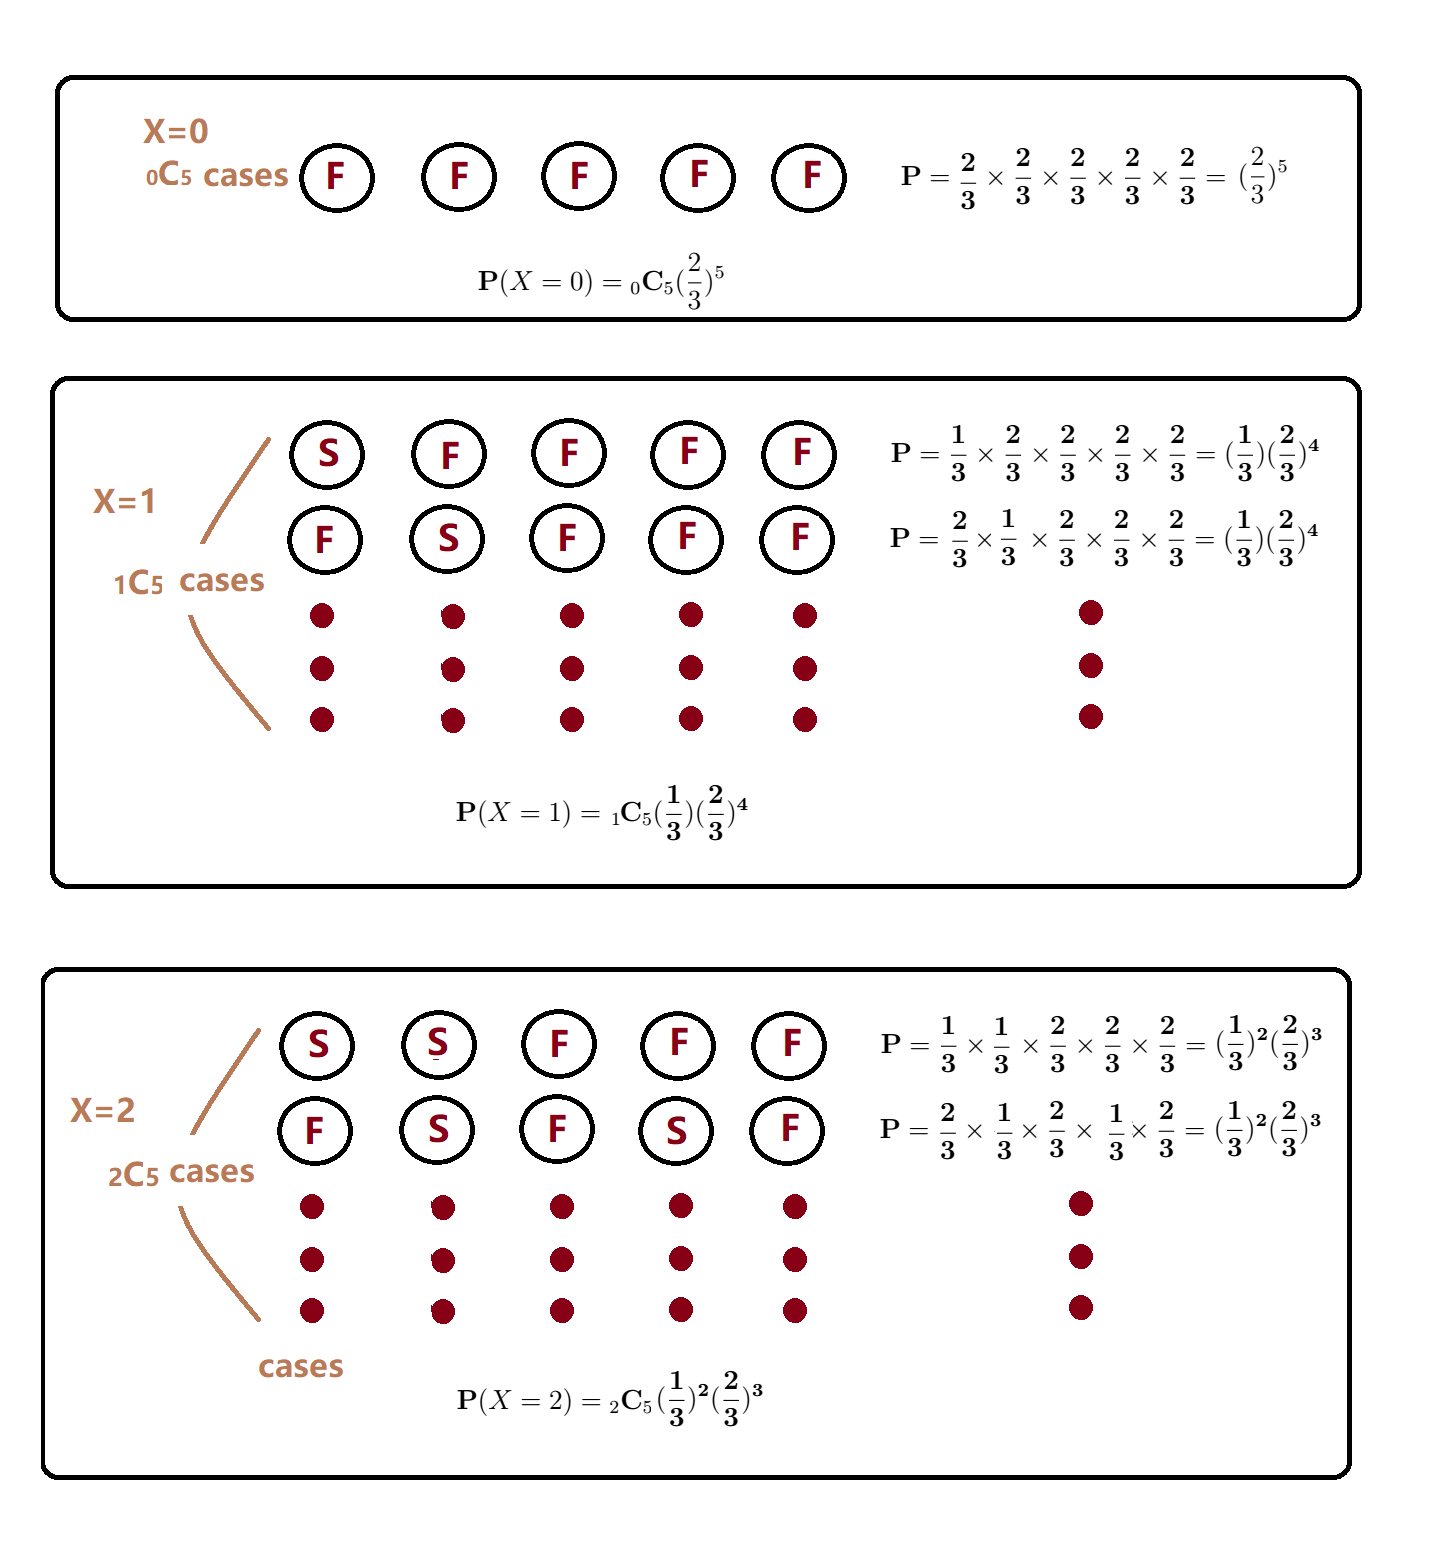
\includegraphics[scale=0.6]{BinomialDistribution}
       \caption{The distribution of binomial distribution}
       \label{BinomialDistribution}
   \end{figure}
   
   Generalize the results in figure \ref{BinomialDistribution}, we have the binomial probability formula for $X \sim B(n, p)$:
       $$\textbf{P}(X=k) = {}_k\textbf{C}_n p^k(1-p)^{(n-k)}, \qquad k = 0,\,1\, \cdots, \, n$$
       \colorbox{babypink}{\parbox{\textwidth}{
        The binomial random variable $X \sim N(n, p)$ is a discrete random variable and takes values $\{0, 1, 2, \cdots, n\}$. The distribution is symmetric and unimodal(one peak), with mode around $\displaystyle{\frac{n+1}{2}}$.
       }}
       
       \newpage
        
       \noindent\textbf{Mean ,Variance  and standard deviation}\vspace{0.6cm}\\
       $X\sim N(n,p)$, means $X$ is the number of success among $n$ trials with the probability of success for each trial $p$. Define a new random variable $X_i$ as the number of success of the $i$th trial. The distribution of $X_i$, $\textbf{Var}(X_i)$ and $\textbf{E}(X_i)$ are given below.
       \begin{table}[H]
       \centering
           \begin{tabular}{ccc}
               \hline
               $X_i$&0&1\\
               \textbf{Probability:}&$1-p$&$p$\\
               \hline
           \end{tabular}
       \end{table}

    \begin{textblock}{4}(-3, -1.5)
    \noindent Calculate $\textbf{E}(X_i)$ and $\textbf{Var}(X_i)$.
    \end{textblock}
     $$\textbf{E}(X_i)=p \qquad \textbf{Var}(X_i) = p(1-p).$$
     \vspace{0.3cm}\\
     
     $X$ can be expressed as the sum of  $X_i$s.
     $$X = X_1 + X_2 + \cdots + X_n = \sum _{i-1}^n X_i$$
     \vspace{0.3cm}\\
     According to formulas in \textbf{1.3},
     $$\textbf{E}(X) = \sum _{i-1}^n  = np, \quad \textbf{Var}(X) = \sum _{i-1}^n p(1-p) = np(1-P), \quad \sigma_X = \sqrt{np(1-p)}.$$
     \vspace{0.6cm}\\
 
       \noindent \colorbox{champagne}{\parbox{\textwidth}{
       \textbf{Applying the torque}\vspace{0.3cm}\\
        A machine fastens plastic screw-on caps onto containers of motor oil. If the machine applies more torque than the cap can withstand, the cap will break. Both the torque applied and the strength of the caps vary. The capping-machine torque T follows a Normal distribution with mean 7 inch-pounds and standard deviation 0.9 inch-pounds. The cap strength C (the torque that would break the cap) follows a Normal distribution with mean 10 inch-pounds and standard deviation 1.2 inch-pounds. \vspace{0.3cm}\\
        Now this machine fastened plastic screw\textendash on caps onto 10 containers, What is the probability that no more than 1 caps are broken?
       }}
     \newpage
     
     
      \noindent \textbf{$10\%$ condition}\vspace{0.3cm}\\
       
       In binomial setting, the trials have to be independent, and this strongly restrict the application of binomial distribution. In fact, when those trials are "roughly independent"", binomial distribution can be applied and give a relative good result. When those trials are "roughly independent"?\vspace{0.3cm}\\
       Suppose, we have a bag of balls, the total number is denoted as $N$, and 20\% of them are black, the others are white. Randomly take 2 out of those $N$ balls. Let $\textbf{C}_1$ be the color of the first ball, and $\textbf{C}_2$ the color of the second ball. Take a look at the following conditional probabilities.
       
       $$N=5, \quad\qquad P(\textbf{C}_2 = \text{black}\,|\, \textbf{C}_1 = \text{black}) = 0, \quad P(\textbf{C}_2 = \text{black}\,|\, \textbf{C}_1 = \text{white}) = \frac{1}{4}$$       
             $$N=10, \quad\qquad P(\textbf{C}_2 = \text{black}\,|\, \textbf{C}_1 = \text{black}) = \frac{1}{9}, \quad P(\textbf{C}_2 = \text{black}\,|\, \textbf{C}_1 = \text{white}) = \frac{2}{9}$$              
              $$N=20, \qquad P(\textbf{C}_2 = \text{black}\,|\, \textbf{C}_1 = \text{black}) = \frac{3}{19}, \quad P(\textbf{C}_2 = \text{black}\,|\, \textbf{C}_1 = \text{white}) = \frac{4}{19}$$              
              $$N=40, \qquad P(\textbf{C}_2 = \text{black}\,|\, \textbf{C}_1 = \text{black}) = \frac{7}{39}, \quad P(\textbf{C}_2 = \text{black}\,|\, \textbf{C}_1 = \text{white}) = \frac{8}{39}$$             
               $$N=80, \qquad P(\textbf{C}_2 = \text{black}\,|\, \textbf{C}_1 = \text{black}) = \frac{15}{79}, \quad P(\textbf{C}_2 = \text{black}\,|\, \textbf{C}_1 = \text{white}) = \frac{16}{79}$$       
       \vspace{0.3cm}      
         
  \noindent The difference between $P(\textbf{C}_2 = \text{black}\,|\, \textbf{C}_1 = \text{white})$ and $P(\textbf{C}_2 = \text{black}\,|\, \textbf{C}_1 = \text{black})$ decreases from $\displaystyle{\frac{1}{4}}$ to $\displaystyle{\frac{1}{79}}$ as $N$ increases from 5 to 80. This can be interpreted as "the probability  that $\textbf{C}_1 = \text{black}$ becomes less and less influenced by the values of $\textbf{C}_2$". Loosely speaking, "as $N$ increases, $\textbf{C}_1$ and $\textbf{C}_2$ become more independent". Thus comes the following.\vspace{0.3cm}\\
  \colorbox{babypink}{\parbox{\textwidth}{
  Let $N$ be the population size and $n$ the sample size. If $n \leq 10\%\,N$, then the individuals in the sample are roughly independent. \vspace{0.3cm}\\
  "$\mathbf{n \leq 10\%\,N}$" is called \textbf{the 10\% condition}.
  }}
  \vspace{0.6cm}
  
  \noindent \colorbox{champagne}{\parbox{\textwidth}{
  \textbf{Bad Flash Drives}\vspace{0.3cm}\\
  A supplier inspects an SRS of 10 flash drives from a shipment of 10,000 flash drives. Suppose that (unknown to the supplier) 2\% of the flash drives in the shipment are defective. \vspace{0.3cm}\\
  Find the probability that no more than 2 of the flash drives are defective.
  }}
       \newpage
       
      \noindent \textbf{Approximation of binomial distribution}\vspace{0.6cm}\\
      
      In the formula of the binomial distribution
      $$\textbf{P}(X=k) = {}_k\textbf{C}_n p^k(1-p)^{(n-k)},$$
      as $n$ increase, the difficulty of computation of $\textbf{P}(X=k)$ increase rapidly. However, the binomial distribution can be approximated by normal distribution if \textbf{the large counts condition} is met.\vspace{0.3cm}\\
      \colorbox{babypink}{\parbox{\textwidth}{
     If  $X \sim N(n, p)$, $np \leq 10$ and $n(1-p) \leq 10$, then the distribution of $X$ can be approximated by $N(\mu_X, \sigma_X)$, where $\mu_X=np, \quad \sigma_X = \sqrt{np(1-P}$. \vspace{0.3cm}\\
     The condition "$np \leq 10$ and $n(1-p) \leq 10$" is called \textbf{large counts condition}.
      }} \vspace{0.6cm}\\
      \colorbox{champagne}{\parbox{\textwidth}{
      \textbf{Checking for Survey Error}\vspace{0.3cm}\\
      One way of checking the effect of undercoverage, nonresponse, and other sources of error in a sample survey is to compare the sample with known facts about the population. About 12\% of American adults identify themselves as black. Suppose we take an SRS of 1500 American adults and let X be the number of blacks in the sample.
      \begin{enumerate}[(a)]
          \item Show that X is approximately a binomial random variable.
          \item Check the conditions for using a Normal approximation in this setting.
          \item Use a Normal distribution to estimate the probability that the sample will contain between 165 and 195 blacks
      \end{enumerate}
      }}
      \newpage
      
  \section{Geometry random variables}  
Take a look at the following setttings.
\begin{enumerate}[(1)]
    \item Roll a die till you get double. \textbf{X} is  the number of rolls
    \item Toss a coin till you get a head. \textbf{Y} is the number of tosses.
\end{enumerate}
In the above setting, the outcomes of each outcome is binary, either "success" or "failure". The trials are independent. The probability of "success" among all trials is a constant. However, we don't know the number of trials in advance, and the number of trials are defined as random variables \textbf{X} and \textbf{Y} in the above two setting. \textbf{X} and \textbf{Y} are called \textbf{Geometric random variables}\vspace{0.6cm}\\

\colorbox{champagne}{\parbox{\textwidth}{
\textbf{Deduce the formulas}\vspace{0.3cm}\\
Suppose \textbf{X} is a \textit{geometric random variable} with probability of success $p$.\vspace{0.3cm}\\
Find $\textbf{P}(X = k)$ and $\textbf{E}(X)$.
}}


     

\end{document}